\section{Parallelism}
Speedup:
$$S(n) = \frac{T(1)}{T(n)}$$
Ahmdahl's law:
$$ S(n) = \frac{1}{(1 - p)+\frac{p}{n}}$$
wobei $p$ der parallelisierbare Anteil ist (in \%)
\subsection{Deadlocks}
\paragraph{Coffman conditions}
\begin{enumerate}
	\item Mutual Exclusion
	\item Hold and wait
	\item No preemption
	\item Circular wait
\end{enumerate}
All of these conditions must apply for a deadlock to be possible
\subsection{Livelocks}
Threads switching but not making any progress
\subsection{Starvation}
Occurs if a thread cannot aquire any resources even if no deadlocks exist

\subsection{Flynn's taxonomy}

\begin{enumerate}
	\item SISD: Single instruction x single data
	\item SIMD: Single instruction x multiple data
	\item MIMD: Multiple instruction x multiple data	
	\item MISD: Multiple instruction x multiple data
\end{enumerate}

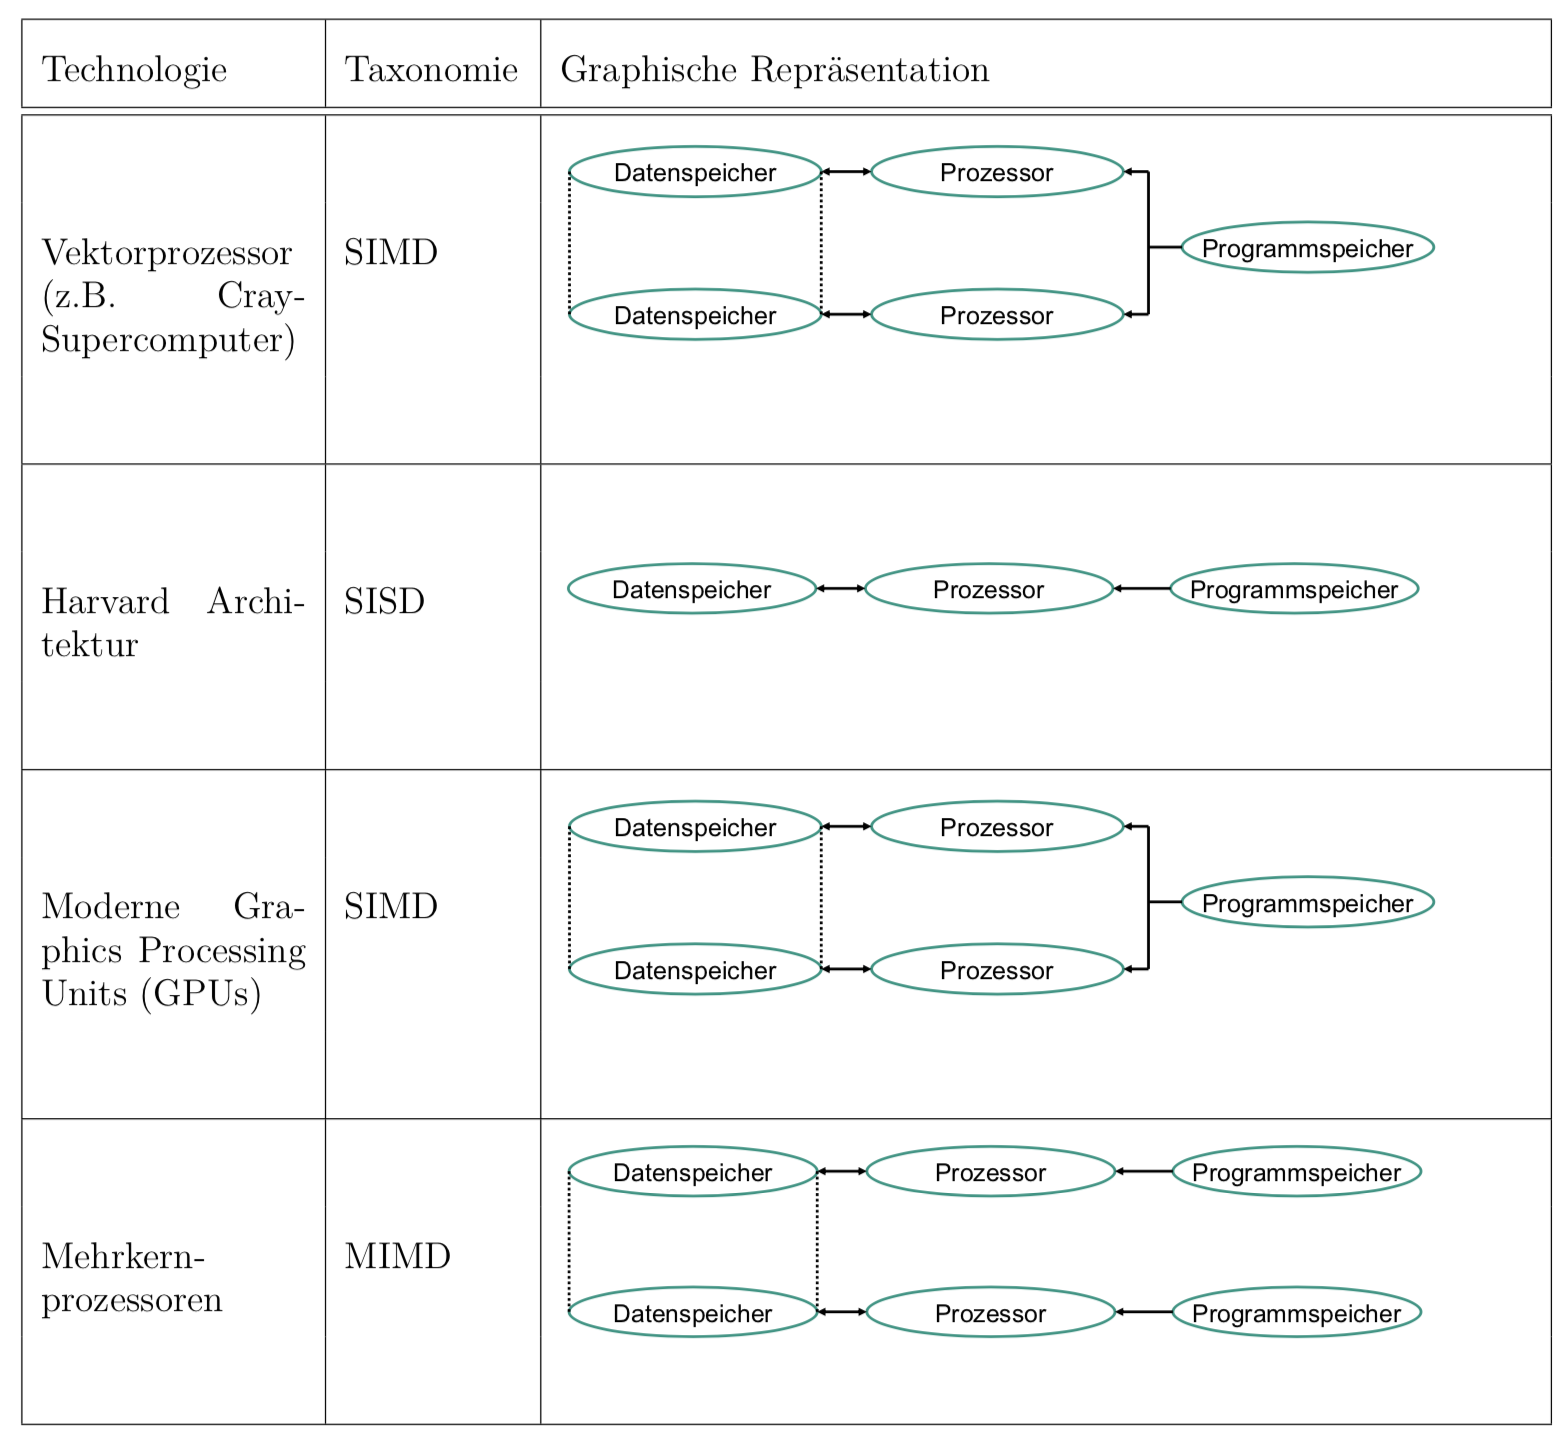
\includegraphics[width=\columnwidth]{images/flynn.png}